\documentclass{standalone}
\usepackage{tikz}
\usetikzlibrary{patterns}

\begin{document}
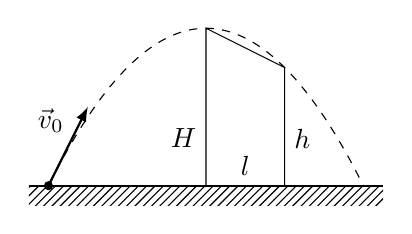
\begin{tikzpicture}    
	\draw [draw=none, pattern=north east lines] (-0.25,0) rectangle (4.25,-0.25);
	\draw [thick] (-0.25,0) -- (4.25,0);
	\draw [fill] (0,0) circle (0.05);
	\draw (2, 0) -- (2, 2) -- (3, 1.5) -- (3, 0);
	\draw [dashed]  plot[smooth,domain=0:4] (\x, {0.5*(4-(\x))*(\x)});
	\node [left] at (2, 0.6) {$H$};
	\node [right] at (3, 0.6) {$h$};
	\node [above] at (2.5, 0) {$l$};
	\draw [arrows={-latex}, thick] (0, 0) -- (0.5, 1) node [above=-5pt, left=5pt] {$\vec{v}_0$};
\end{tikzpicture}
\end{document}